\documentclass[runningheads]{llncs}

\usepackage{graphicx}
\usepackage{float}
\usepackage{bookmark}
\bookmarksetup{
  open,
  addtohook={%
    \ifnum\bookmarkget{level}<1 %
      \bookmarksetup{bold}%
    \fi
  },
}

\begin{document}

\title{Static PE Malware Detection using Gradient Boosting Decision Trees algorithm}
\titlerunning{Static PE Malware Detection using GBDT}

\author{Huu-Danh Pham\inst{1} \and Thanh-Nguyen Vu\inst{1}}
\authorrunning{H.D. Pham and T.N. Vu}

\institute{Vietnam National University Ho Chi Minh City, \\
University of Information Technology, Ho Chi Minh City, Vietnam \\
\email{\{14520134,nguyenvt\}@uit.edu.vn}}
%
\maketitle              % typeset the header of the contribution
%

\begin{abstract}
Static malware detection is an essential layer in a security suite, which attempts to classify samples as malicious or benign before execution. 
However, most of the related works incur the scalability issues, for examples, methods using neural networks usually take a lot of training time \cite{raff2017malware}, or use imbalanced datasets \cite{saxe2015deep,vu2017metamorphic}, which makes validation metrics misleading in reality.  In this study, we apply a static malware detection method by Portable Executable analysis and Gradient Boosting Decision Tree algorithm. 
We manage to reduce the training time by appropriately reducing the feature dimension. 
The experiment results show that our proposed method can achieve up to 99.394\% detection rate at 1\% false alarm rate, and score results in less than 0.1\% false alarm rate at a detection rate 97.572\%, based on more than 600,000 training and 200,000 testing samples from Endgame Malware BEnchmark for Research (EMBER) dataset \cite{anderson2018ember}.

\keywords{Malware detection \and Machine learning  \and PE file format \and Gradient boosting decision trees \and EMBER dataset.}
\end{abstract}
%
%
%
\section{Introduction}

Malware is typically used as a catch-all term to refer to any software designed to cause damage to a single computer, server, or computer network.  
A single incident of malware can cause millions of dollars in damage, i.e., zero-day ransomware WannaCry has caused world-wide catastrophe, from knocking U.K. National Health Service hospitals offline to shutting down a Honda Motor Company in Japan \cite{chen2017automated}. 
Furthermore, malware is becoming more sophisticated and more varied everyday. 
Accordingly, the detection of malicious software is an essential problem in cybersecurity, especially as more of society becomes dependent on computing systems.

Malware detection methods can be classified in either static malware detection or dynamic malware detection \cite{egele2012survey}. 
Static malware detection classifies samples as malicious or benign without executing them, in contrast to dynamic malware detection which detects malware based on its runtime behavior. 
In theory, dynamic malware detection provides the direct view of malware action, is less vulnerable to obfuscation, and makes it harder to reuse existing malware \cite{moser2007limits}. 
But in reality, it is hard to collect a dataset of malware behavior because the malwares can identify the sandbox environment and prevent itself from performing the malicious behavior. 
In contrast, although static malware detection is known to be undecidable in general \cite{cohen1987computer}, it has enormous datasets which can be created by aggregating the binaries files, and is a critical layer in a security suite because when successful, it allows identifying malicious files before execution.

In this study, we present and optimize a static malware detection method using hand-crafted features derived from parsing the PE files and Gradient Boosting Decision Trees (GBDT), a widely-used powerful machine learning algorithm.
Rather than using raw binary files, our proposed method use the statistical summaries to decrease the privacy concerns of various benign files and makes it easy to request the balanced dataset. 
GBDT also shows its efficiency and accuracy by taking less time for training and achieving impressive evaluation results.

\section{Related Work}

Malware detection has grown over the past several years, due to the more rising threat posed by malware to large businesses and governmental agencies. 
Various machine learning-based static Portable Executable (PE) malware detection methods have been proposed since at least 1995 \cite{kephart1995biologically,schultz2001data,kolter2006learning,saxe2015deep,raff2017malware}. 
In 2001, Schultz et al. represented PE files by features that included imported functions, strings, and byte sequences \cite{schultz2001data}. In 2006, Kolter et al. used byte-level N-grams and techniques from natural language processing, including TFIDF weighting of strings to detect and classify malicious files \cite{kolter2006learning}. In 2015, Saxe and Berlin  leveraged novel by using a histogram of byte entropy values for input features and a multi-layer neural network for classification \cite{saxe2015deep}. In 2017, Edward Raff et al. showed that fully connected and recurrent networks could be applied in the malware detection problem \cite{raff2017learning}. They also extends those results by training end-to-end deep learning networks on entire, several million byte long executables, and encounters a wide breadth of potential byte content \cite{raff2017malware}.

In Vietnam, Nguyen Van Nhuong et al. proposed a semantic set method to detect metamorphic malware in CISIM 2015 \cite{van2014semantic}. Vu Thanh Nguyen et al. proposed a combined method of Negative Selection Algorithm and Artificial Immune Network for virus detection in in FDSE 2014 \cite{nguyen2014combination}, and a metamorphic malware detection system by Portable Executable Analysis with the Longest Common Sequence in FDSE 2017 \cite{vu2017metamorphic}.

\section{Proposed Method}

\subsection{The Issues of using Imbalanced Dataset}

Most of the related work use the imbalanced dataset \cite{saxe2015deep,vu2017metamorphic}. For examples, Saxe and Berlin used the dataset of 431,926 binaries which consists 350,016 malicious files \cite{saxe2015deep}, Vu Thanh Nguyen et al. used the dataset of 9690 files which only has 300 benign files \cite{vu2017metamorphic}. 

In fact, the number of malicious files is often much more massive than the number of benign files because almost benign binaries are often protected by the copyright laws which do not allow for sharing. This makes malware identification problem become different from other machine learning classification problems, which commonly have fewer samples in important classes. Further, the size of the dataset is usually not large enough because the malware analysis and data labeling are consuming processes that required well-trained security engineers. There are also many risks in publishing a large dataset that includes malicious binaries. 

Using imbalanced datasets can make validation metrics misleading.
For examples, with 96.9\% of data is malicious files, a model that labels all samples as malware achieves 96.9\% accuracy, 96.9\% precision (P), 100\% recall (R) and 0.9843 F-score ($F =  2PR / (P + R) $ \cite{chinchor1992muc}).
It also give way to false positives, which cause negative user experiences.
According to a survey of IT administrators in 2017, 42 percent of companies assume that their users lost productivity as an issue of false-positive results, which creates a choke point for IT administrators in the business life cycle \cite{jonathan2017survey}.

\subsection{Feature Extraction}

By using the simple feature extraction methods inspired by the EMBER dataset owners rather than raw binary files, collecting data is not affected by privacy policies and its is much more easier to get a balanced dataset. By conducting many experiments, we decrease the feature dimension by 30 percent (1711 instead of 2351) to reduce the training time but still manage to achieve a better evaluation results. In detail, we extracted each Portable Executable file into eight feature groups which can be classified into two types: format-agnostic features (byte-entropy histogram, byte histogram and string information) and parsed PE features. File-format agnostic feature groups decrease privacy concerns while parsed PE feature groups encapsulates the information related to executable code.

\subsubsection{Byte-Entropy Histogram}

The work \cite{saxe2015deep} shows that, in practice, representing byte values in the entropy context in which they occur separates byte values from the context effectively. For example, x86 instruction data from byte values occurring in compressed data. To compute the byte-entropy histogram, we slide a 2048-length window over all the input bytes with a step size of 1024 bytes. Use a simple trick to calculate the entropy $H$ faster, i.e., reducing the information by half, and pairing it with each byte within the window. Then, we compute a two-dimensional histogram with $16 \times 16$ bins that quantize entropy and the byte value. Finally, row vectors in the matrix are concatenated and normalized the final 256-value vector.

\subsubsection{Byte Histogram}

The byte histogram is a 256-value vector which represents the distribution of each byte value within the file.

\subsubsection{String Information}

The final format-agnostic group of features is string information. These features are derived from the printable sequences of characters in the range \verb|0x20| to \verb|0x7f|, that have at least five characters long. We use the number of strings, the average length of these strings, the amounts of lines  that may sequentially indicate a path (begin with \verb|C:\|), an URL(start with \verb|http://| or \verb|https://|), a registry key (the occurrences of \verb|HKEY_|) and a bundled executable (the short string \verb|MZ|). Also, we use a histogram of the printable characters within these strings.

\subsubsection{Parsed PE Features}

Five other feature groups are delivered from parsing the Portable Executable file format. The first group is the general information group, which includes the file size and necessary information collected from the PE header (the virtual size of the file, the number of imported and exported functions, the number of symbols, whether the data has a debug section, thread local storage, resources, relocations, or a signature). The second group is the information from Common Object File Format header (the timestamp in the header, the target machine and a list of image characteristics) and from the optional header (target subsystem, DLL  characteristics,  the file magic as a string, major and minor image versions, linker versions, system versions and subsystem versions, and the code size, header size and commit size). The next two feature groups are imported and exported functions. we apply the 512-bin hashing trick to capture individual imported functions, by representing it in string format \verb|library:function|, for example, \verb|kernel32.dll:CreateFileMappingA|. Simarly, a list of the exported functions is hashed into a list of 128-value vectors. The last group contains section information, i.e., the name, size, entropy, virtual size, and a list of strings representing section characteristics.

\subsection{Gradient Boosting Decision Trees}

For classification, we propose the method which uses the traditional Gradient Boosting Decision Trees (GBDT) algorithm with 400 iterations and 64 leaves in one tree. In the training step, we configure that there must be at least 200 samples in one child, and set learning rate at 5 percent. The reasons for choosing GBDT are below.

\subsubsection{Scalability}

There are many essential features that is need to classify malicious and benign files. Even after feature selection, the massive number of features causes scalability issues for many machine learning algorithms. For example,  non-linear  SVM  kernels require $O(N^2)$ multiplication during each iteration, and k-Nearest Neighbors (k-NN) requires significant computation and storage of all label samples during prediction. Accordingly, scalable alternatives are used in malware detection, and the two most popular algorithms are neural networks and ensemble decision trees.

\subsubsection{Training time}

One of the most challenges that anti-malware systems usually have is the enormous amounts of data which needs to be evaluated for possible malicious intent \cite{ronen2018microsoft}. Those results will be used to train the model to automatically evaluate samples in future. Hence, the training time becomes the essential criteria. Using neural networks usually take a long time for training. For examples, MalConv, the end-to-end deep learning model \cite{raff2017malware}, took 25 hours for each epochs in training with the binaries from EMBER dataset \cite{anderson2018ember}. In contract, tree ensemble algorithms handle very well a large number of training samples in moderate training times. One of popular tree ensemble algorithms, which has shown its effectiveness in several challenges, is gradient boosting decision tree. GBDT is widely-used and achieves state-of-the-art performances in many tasks, such as ranking \cite{chris2010ranknet} and click prediction \cite{richardson2007predicting}. Besides, Guolin Ke et al. recently release LightGBM, which is a highly efficient gradient boosting framework that speeds up the training process up to over 20 times while achieving almost the same accuracy \cite{ke2017lightgbm}.

\section{Experiment}

\subsection{Dataset}

In our experiment, we use 600,000 labeled training samples and 200,000 testing samples from Endgame Malware BEnchmark for Research (EMBER) dataset \cite{anderson2018ember}.

\begin{figure}[H]
\centering
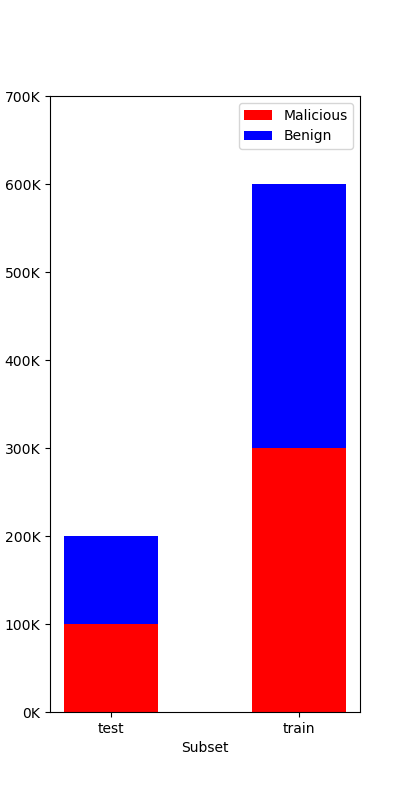
\includegraphics[scale=0.4]{dataset.png}
\caption{Distribution of samples in EMBER dataset.}
\label{fig:ember}
\end{figure}

\subsection{Evaluation Criteria}

\subsubsection{False Alarm Rate}

False positives, or false alarms, happen when a detector mistakes a malicious label for a benign file. We intend to make the false positive rate as low as possible, which is untypical for machine learning application. It is important because even one false alarm in a thousand benign files can create severe consequences for users. This problem is complicated by the fact that there are lots of clean files in the world, they keep appearing, and it is more challenging to collect these files. We evaluate the accuracy of our method at two specific false alarm rate values: at less than 0.1\%, and at less than 1\%.

\begin{center}
    ${False\ alarm\ rate} =  \frac{\sum False\ positive}{\sum Condition\ negative}$
\end{center}

\subsubsection{Detection Rate}

The detection rate, (eqv. with recall or true positive rate), measures the ratio of malicious programs detected out of the malware files used for testing. With higher recall, fewer actual cases of malware go undetected.

\begin{center}
    ${Detection\ rate} =  \frac{\sum True\ positive}{\sum Condition\ positive}$
\end{center}

\subsubsection{Area Under the ROC curve}

The Area Under the ROC curve, AUROC or AUC for short, provides an aggregate measure of performance across all possible classification thresholds. AUC is scale-invariant and measures how well predictions are ranked, rather than their absolute values. Besides, AUC is classification-threshold-invariant, so that it can measure the quality of the predictions irrespective of what threshold is chosen. A model whose predictions are 100\% wrong has an AUC of 0.0, and the one whose predictions are 100\% correct has an AUC of 1.0.

\subsection{Experimental Results}

The proposed GBDT-based malware detection method is implemented with LightGBM framework \cite{ke2017lightgbm}, and the input feature vectors have dimension of 1711. All our experiments were run on an instance which has 24 vCPUs and 32 GB memory. Using parallel programming, it took about 10 minutes to vectorize the raw features and about 5 minutes to train the model. The ROC curve of the final model is shown in Figure \ref{fig:roc_curve_with_highlights}.

\begin{figure}[h]
\centering
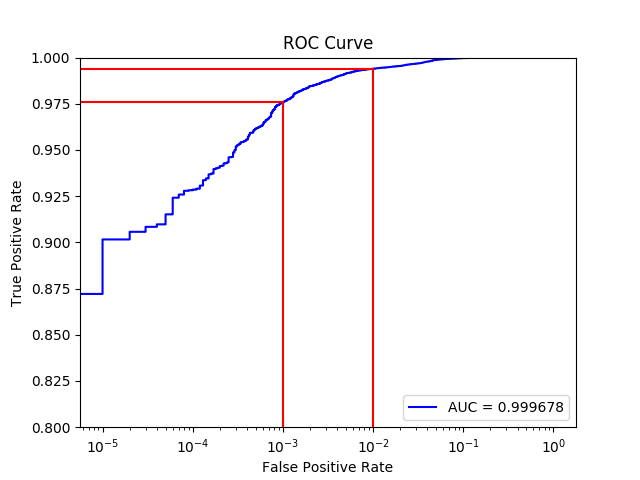
\includegraphics[width=\textwidth]{roc_curve_with_highlights.png}
\caption{The ROC curve of proposed model}
\label{fig:roc_curve_with_highlights}
\end{figure}

The area under ROC curve exceeds $0.999661$, which means that almost all the predictions are correct. With a threshold of $0.828987$, the model score results in less than $0.1\%$ false alarm rate at a detection rate $97.5720\%$. At less than $1\%$ false positive rate, the model exceeds $99.3940\%$ detection rate with a threshold of $0.307897$. 

The baseline model has only the area under the ROC curve of $0.999678$, score results in less than $0.1\%$ FPR at TPR exceeding $92.99\%$, and at less than $1\%$ FPR, it exceeds $98.2\%$ TPR. Our model has better performance because of hyper-parameter tuning, and it also takes less time for training as a result of reducing feature space. Evidently, the model has better performance than the MalConv model trained on the raw binaries \cite{anderson2018ember}, which has ROC AUC is 0.99821, corresponding to a 92.2\% TPR at a FPR less than 0.1\%, and a 97.3\% TPR at a less than 1\% FPR.

\section{Conclusion and Future Works}

In this study, we show the weakness in earlier proposed methods, especially the issues in using imbalanced datasets in malware detection. 
We demonstrate feature extraction using file-format agnostic features decreases privacy policies and makes it easier to collect benign files. 
We have also applied a method for static PE malware detection using gradient boosting decision trees algorithm. 
On the EMBER dataset, our proposed model achieve a better performance than the baseline model introduced by the dataset owners while takes less training time by reducing the feature vector dimension. 
Besides, the validation results reinforce the evidence that leveraging domain knowledge from parsing the PE format file has still achieved a remarkable performance.

The study conducted in this project was a proof-of-concept, and we can identify some future developments related to the practical implementation.

\subsubsection{Reduce the feature space}

There is possible to reduce the dimension of feature vectors. Input vectors with smaller size boost the model and take less training time. 

\subsubsection{Use other datasets}

Although the EMBER dataset is broad, covering most of the malware species, it does not include all possible kinds. Collecting a dataset is a task that requires a lot of time and efforts, especially in malware detection domain. With using format-agnostic features, we can receive more samples from security organizations in future. 

\bibliographystyle{splncs04}
\bibliography{references}

\end{document}